\section{实验分析与结果分析}
本章将对研究过程中的重要实验进行说明和分析。在文本主题分析的实验中,将分别对基于标签的长文本主题识别算法以及基于弹幕的视频精彩镜头提取方法进行评估。在用户兴趣模型的实验中,将对基于SICT和DIST的兴趣相似度匹配算法进行评估。在兴趣覆盖网络的实验中,将对基于用户兴趣集的资源传播方法进行评估。

\subsection{文本主题分析的实验与评价}
这一节主要对文本资源的主题进行分析,为了说明主题在文本特征表示上的作用十分突出,这里先从文本分类问题开始对主题有一个直观上的认识。

首先,对于分类的数据集,选择的是著名的20 News Group\footnote{http://qwone.com/~jason/20Newsgroups/},并且是已经去重的后的数据,包括了18828篇文档,几乎均匀地分成了20个类,6个学科大类,如图\ref{fig:20news}所示。因为是有监督的分类问题,所以选取80\%作为训练数据,剩下20\%作为测试数据。
\begin{figure}[!ht]
\centering
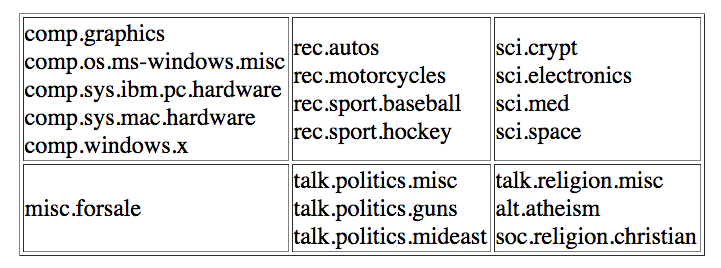
\includegraphics[width=0.9\textwidth]{20news.png}
\caption{20 News Group的分类}
\label{fig:20news}
\end{figure}

接着,这里选择两种用于描述文档的特征:基于词频的向量和基于主题的向量。在计算词频特征的时候,需要对训练集进行分词、去除英文的标点和停顿词,然后每个文档表示成一个向量,向量中的每个值为单词在文档中出现的数量与文档单词总数量的比值。而计算主题向量的时候,这里采用LDA模型进行计算,主题个数取为10,经过训练后得到的文档-主题矩阵和主题-单词矩阵,这里选择文档-主题矩阵中的每一行作为一篇文档的特征向量。

然后,这里选取了三个分类算法:AdaBoost、最大期望算法(Expectation Maximum algorithm)、朴素贝叶斯分类器(Naive Bayes Classifer)。其中AdaBoost由Icsiboost-bigram\footnote{www.mlcomp.org}实现,这是一个基于一层决策树的AdaBoost,通过把弱分类器整合在一起从而生成一个强分类器。最大期望算法主要用于文档的分类,通过迭代技术来找到最大的后验概率,从而决定分类器的参数。朴素贝叶斯分类器则是根据贝叶斯定理,在词袋和条件独立的假设下,在给定分类的条件下使单词的联合概率最大。

\begin{table}[!hbt]
  \centering
  \caption{基于词频特征和主题特征的文本分类实验}
  \begin{tabular}{|c|c|c|c|}
    \hline
    算法 & AdaBoost & EM & Naive Bayes \\
    \hline
    准确率(词频)& 71.6\% & 78.9\% & 86.2\% \\
    \hline
    准确率(主题)& 75.4\% & 83.3\% & 90.9\% \\
    \hline
  \end{tabular}
  \label{tbl:classify}
\end{table}

如表\ref{tbl:classify}所示,当文档用主题向量来表示的时候,准确率提高了4\%左右的提升,因此可以看出,本文基于主题模型对文本进行分析是有据可循的。

\subsubsection{基于标签的长文本主题识别算法}
这一节将对基于LDA和L-LDA两种主题模型的分类问题进行实验,从而来看两者在标签的标记上的区别。

数据集将选择两个进行比较,一个依然是20 News Group。另一个数据集选取了复旦大学中文语料库,该语料库共分为20类,但是每一类中的文章数量是不均匀的,即会出现有的类很多文档,有的类很少,可以说这点比较符合现实。如表\ref{tbl:fudan}所示为各个类中文档的数量(从高到低排序)。
\begin{table}[!hbt]
  \centering
  \caption{复旦大学中文语料库的统计信息}
  \begin{tabular}{|lll|lll|}
    \hline
    类别名称 & 代码 & 文档数量 & 类别名称 & 代码 & 文档数量 \\
    \hline
    Economy & C34 & 3201篇 & Education & C5 & 120篇 \\
    Computer & C19 & 2715篇 & Transport & C29 & 116篇 \\
    Sports & C39 & 2507篇 & Medical & C36 & 104篇 \\
    Enviornment & C31 & 2435篇 & Law & C35 & 103篇 \\
    Politics & C38 & 2050篇 & Philosophy & C6 & 89篇 \\
    Agriculture & C32 & 2043篇 & Literature & C4 & 67篇 \\
    Art & C3 & 1482篇 & Mine & C23 & 67篇 \\
    Space & C11 & 1282篇 & Energy & C15 & 65篇 \\
    History & C7 & 934篇 & Electronics & C16 & 55篇 \\
    Military & C37 & 150篇 & Communication & C17 & 52篇 \\
    \hline
  \end{tabular}
  \label{tbl:fudan}
\end{table}

这里的性能评价指标使用$F_1$,表示在数据集上整体分类算法的性能:
\begin{equation}
  F_1=2\cdot \frac{precision\cdot recall}{precision+recall}
\end{equation}

对于复旦大学中文语料库,分别对每个类取2至8个主题,并用LDA和L-LDA进行训练得到主题向量,然后计算$F_1$,可以得到表\ref{tbl:classify2}的结果。从中可以看到两点,第一,L-LDA总体的性能要好于LDA;第二,LDA的性能几乎不会随着主题数量的增加而变化,但是L-LDA的性能会随着主题数量的增加而变好。

\begin{table}[!hbt]
  \centering
  \caption{基于复旦大学语料库的LDA与L-LDA的性能比较}
  \begin{tabular}{|c|c|c|c|c|c|c|c|}
    \hline
    主题数量 & 2 & 3 & 4 & 5 & 6 & 7 & 8 \\
    \hline
    $F_1$ (LDA) & 85.1\% & 85.7\% & 85.7\% & 85.8\% & 85.8\% & 85.6\% & 85.8\% \\
    \hline
    $F_1$ (L-LDA) & 87.9\% & 88.9\% & 88.7\% & 89.5\% & 90.1\% & 89.9\% &89.6\% \\
    \hline
  \end{tabular}
  \label{tbl:classify2}
\end{table}

在20 News Group语料库中,执行与上面类似的操作,可以得到表\ref{tbl:classify3}的结果。从中可以发现,L-LDA在性能上整体依然比LDA的性能好3\%左右,但是两者都没有随着主题数量的增加有明显变化,导致这个现象的原因可能是因为该语料库中每个分类的文章数量几乎相同。

\begin{table}[!hbt]
  \centering
  \caption{基于20 News Group语料库的LDA与L-LDA的性能比较}
  \begin{tabular}{|c|c|c|c|c|c|c|c|}
    \hline
    主题数量 & 2 & 3 & 4 & 5 & 6 & 7 & 8 \\
    \hline
    $F_1$ (LDA) & 83.8\% & 84.1\% & 84.7\% & 84.6\% & 84.5\% & 84.3\% & 84.3\% \\
    \hline
    $F_1$ (L-LDA) & 87.3\% & 87.3\% & 87.2\% & 87.2\% & 87.1\% & 87.3\% &87.3\% \\
    \hline
  \end{tabular}
  \label{tbl:classify3}
\end{table}

综上所述,基于L-LDA的方法对文本分类效果在整体上比原始的LDA效果更好,但是L-LDA的性能与主题数量和类别中的文本数量有关。所以,在对长文本进行带标签进行识别时,优先利用L-LDA做主题识别,然后再用传统的基于VSM、甚至LDA进行补充。

\subsubsection{基于弹幕的视频精彩镜头提取方法}
在这个实验中,先提出了一个模拟弹幕生成过程的算法\ref{alg:gen_video},并用此算法来生成模拟数据,为之后的模拟实验提供数据。之所以使用模拟数据来进行验证,是因为弹幕视频网站不直接提供精彩镜头,需要花费很长的时间进行人工标注,所以在此先用模拟生成的数据进行实验。

\begin{algorithm}[!bht]
\caption{弹幕模拟生成过程}
\ForEach{all features $f \in [1,K]$}{
  sample feature mixture proportion $\vec{\varphi}_k \sim Dir(\vec{\beta})$
}
\ForEach{all videos $m \in [1,M]$}{
  sample video mixture proportion $\vec{\vartheta}_m \sim Dir(\vec{\alpha})$
  sample video length $L_m \sim Poisson(\lambda_1)$
  two-step highlights simulation~(*)
  \ForEach{all sequential timestamp $t$ of video $m$}{
    sample probability $p \sim uniform(0,1)$
    \If{$t$ is in highlight and $p\in(0,\rho)$}{
      sample feature index $z_{m,t} \sim Mult(\vec{\vartheta}_{m})$
      sample keyword $w_{m,t} \sim Mult(\vec{\varphi}_{z_{m,t}})$
    }
    \ElseIf{$t$ is not in highlight and $p\in(0,1-\rho)$}{
      sample feature index $z_{m,t} \sim
       Mult(\vec{\vartheta}_{m})$
      sample keyword $w_{m,t} \sim Mult(\vec{\varphi}_{z_{m,t}})$
    }
  }
}
\label{alg:gen_video}
\end{algorithm}

利用这个生成过程,首先生成含有2000个词汇的情感词典,并用标示符来表示。如图\ref{fig:keyword_dist}所示,单词出现频率的分布服从正太分布,且它们之和是1。接下来,生成10个从多项分布采样的特征,每个特征都有一定的概率会被选到,如图\ref{fig:feature_dist.png}所示。这些特征之所生成是为了之后模拟弹幕。接着,根据算法\ref{alg:gen_video},生成40000个视频,平均长度为20,平均精彩镜头的数量为4,平均弹幕数量是400。注意到,这里生成的精彩镜头是为了做训练集,之后可以用来与估计的精彩镜头做比较。弹幕的生成过程有一点不一样,因为先要加入噪声数据,来测试我们的方法。有用的弹幕也由同样的过程进行生成,而噪声弹幕是从字典中均匀取出的。

\begin{figure}[!hbt]
  \subfloat[Keywords\label{fig:keyword_dist}]
  {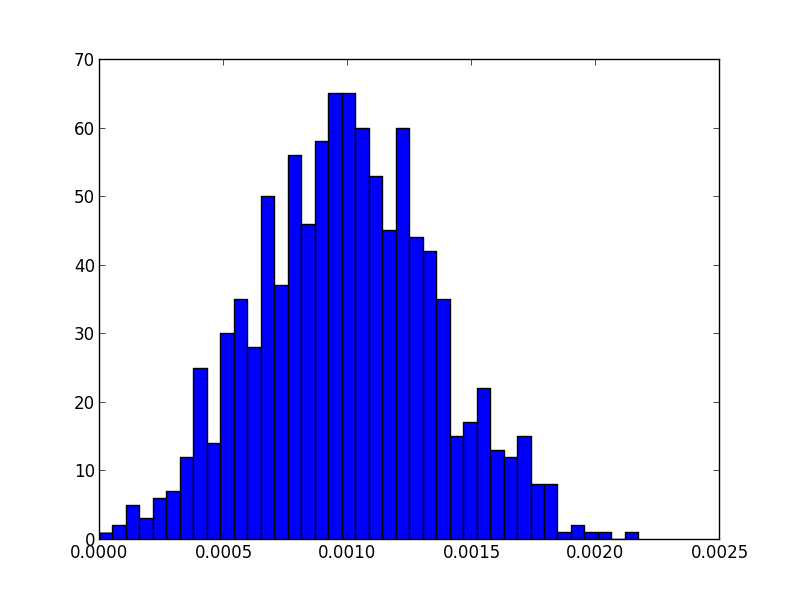
\includegraphics[width=.5\linewidth]{keyword_dist.png}}\hfill
  \subfloat[Features\label{fig:feature_dist}]
  {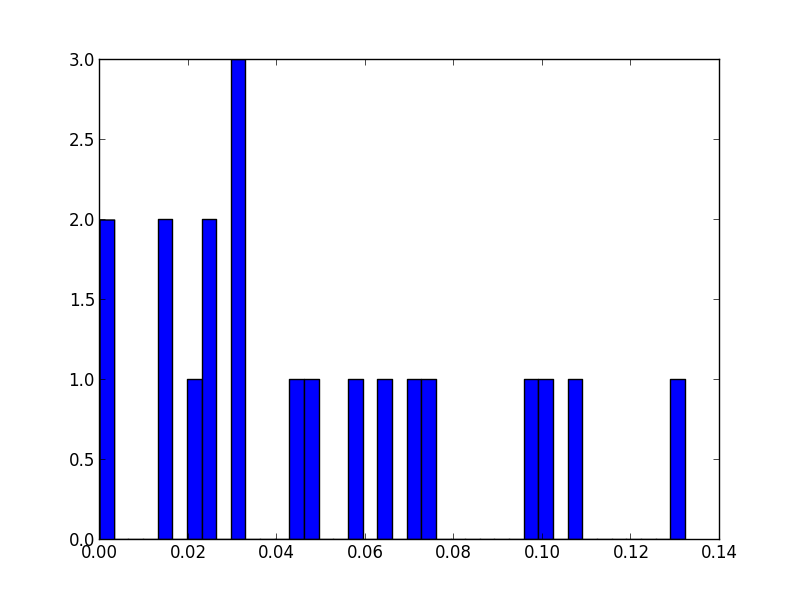
\includegraphics[width=.5\linewidth]{feature_dist.png}}\hfill
\caption{Frequency of different probability}
\end{figure}

这里提出两种评价指标。第一个指标是覆盖率,即判断正确的精彩镜头区间除以真实的精彩镜头区间。基于弹幕的方法,在覆盖率上达到了85.1\%,而传统的基于频率方法的覆盖率只有78.3\%。第二个指标是判断计算出来的特征和原有特征的相似度,相当于给定两个集合,计算他们的最大相似度。

\subsection{基于兴趣树的用户兴趣描述模型的实验与评价}
\subsubsection{基于SICT的兴趣相似度匹配}
\subsubsection{基于DIST的兴趣相似度匹配}

\subsection{兴趣覆盖网络的实验与评价}


\subsection{小结}
